\documentclass{wzuthesis} % 不填充空白页。如果需要双面打印版，请注释掉本行并启用下一行
% \documentclass[print-both-sides]{wzuthesis} % 使用双面打印版（填充额外空白页以保证每一章开头都在奇数页）
\usepackage{mathptmx}
\usepackage{enumitem}
\usepackage{caption}
\usepackage[list=off]{bicaption}

\setmainfont{Times New Roman}[
  Path = ./fonts/,
  Extension = .ttf,
  UprightFont = times,
  BoldFont = timesbd,
  ItalicFont = timesi,
  BoldItalicFont = timesbi
]

\bicaptionsetup[figure]{}{name=Fig.}
\bicaptionsetup[table]{}{name=Table}
\setlength{\headheight}{13pt}

%%===============论文信息=============================
\ctitle{基于XXXXXXXXXXX算法研究} 
                                % 中文题目
\etitle{English Title}                     % 英文题目

\cauthor{WWW}            % 作者姓名
\fen{111}                  % 分类号
\udc{333}                    % UDC
\id{222222222222}               % 学号
\mi{公开}                       % 密级
\xwlx{学术型}                   %学位类型
\pylx{全日制统招研究生}         % 培养类型
\cmajor{计算机科学与技术}       % 专业名称
\cclass{机器学习}              % 研究方向
\cmentor{AGB (教授)} % 指导老师
\cdata{2025年11月8日} %完成时间
\blindcode{} % 盲审代码
%%===================================================
% \def\blind{}       % 盲审版把这条注释打开



\cabstract{
中文摘要应该将学位论文的内容要点简短明了地表达出来，应该包含论文中的基本信息，体现科研工作的核心思想。摘要内容应涉及本项科研工作的目的和意义、研究方法、研究成果、结论及意义。注意突出学位论文中具有创新性的成果和新见解的部分,语言力求精炼，约 500-800 字左右（限一页）。为了便于文献检索，应在本页下方另起一行注明论文的关键词（3-7 个）, 关键词应为公知公用的词和学术术语，不可采用自造字词和略写、符
号等，词组不宜过长。
}
\ckeywords{多变量系统,预测控制,环境试验设备\ 关键词数量为 4-6 个，每一关键词
之间用逗号分开，最后一个关键词后不打标点符号。}

\eabstract{
    % 英文摘要及关键词内容应与中文摘要及关键词内容相同。中英文摘要及其关键词各置一页内。
    英文摘要内容应与中文摘要基本相对应，要符合英语语法，语句通顺，文字流畅,并在其后列出与中文相对应的英文关键词。英文摘要采用第三人称单数语气介绍该学位论文内容，目的是便于其他文摘摘录，因此在写作英文文摘时不宜用第一人称的语气陈述。叙述的基本时态为一般现在时，确实需要强调过去的事情或者已经完成的行为才使用过去时、完成时等其他时态。可以多采用被动语态。中国姓名译为英文时用汉语拼音，按照姓前名后的原则，姓、名均用全名，不宜用缩写。姓全用大写，名的第一个字母大写，名用双中文字时两个字的拼音之间可以不用短划线，但容易引起歧义时必须用短划线。
}
% 英文文关键词(每个关键词之间用,分开, 最后一个关键词不打标点符号。)
\ekeywords{writer recognition,convolutional neural network关键词小写，每一关键词之间用逗号分开，最后一个关键词后不打标点符号。}

\begin{document}
% 论文前置部分
\frontmatter
\makefirstpage
% 如果不需要图、表目录前往cls文件中将相应的注释掉

% 论文主体部分
\mainmatter
\chapter{引言}
文献综述包含的内容：说明论文的主题和选题的范围；对本论文研究主要范围内已有文献的评述；说明本论文所要解决的问题。注意不要与摘要内容雷同。建议与相关历史回顾、前人工作的文献评论、理论分析等相结合，如果引言部分省略，该部分内容在正文中单独成章，标题改为绪论，用足够的文字叙述。注意：是否如实引用前人结果反映的是学术道德问题，应明确写出同行相近的和已取得的成果，避免抄袭之嫌。论文正文是学位论文的主体和核心部分。其行文方式和文体的格局，研究生可根据自己研究课题的表达需要不同而变化，灵活掌握。论文中的计量单位、制图、制表、公式、缩略词和符号必须遵循国家的有关规定。
\newclearpage

\chapter{\LaTeX 模板使用说明}
\section{论文信息的输入和封面的自动生成}
在开始使用本模板前，应该开头位置输入相应的论文相关信息，模板会根据信息自动生成目录和诚信承诺书。如图\ref{author}。
\begin{figure}[htbp]
        \centering
        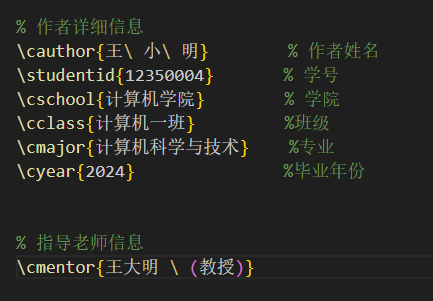
\includegraphics[height=6.54cm]{image/作者信息.png}
        \bicaption{示例图片：数据可视化结果}{Example Figure: Data Visualization Result}
        % \bicaption{示例图片：数据可视化结果}{Example Figure: Data Visualization Result}
        \label{author}
\end{figure}

\section{标题的使用}
标题的使用可见图\ref{til}。其中，一级标题通过\textbackslash chapter\{\}。二级标题通过 \textbackslash section\{\}。三级标题通过\textbackslash subsection\{\}。
\begin{figure}[htbp]
        \centering
        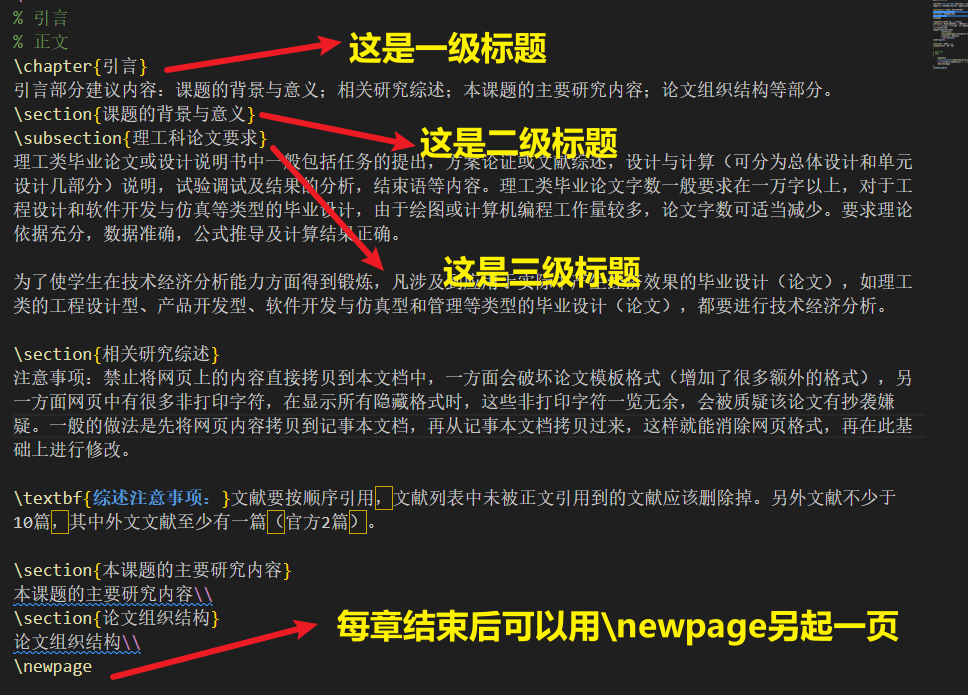
\includegraphics[width=0.65\linewidth]{image/标题使用.png}
        \caption{标题使用}
        \label{til}
\end{figure}

\section{表格的使用}
表格的使用可以通过 \textbackslash table\{\}。详细说明如图\ref{tablea}所示。
\begin{figure}[htbp]
        \centering
        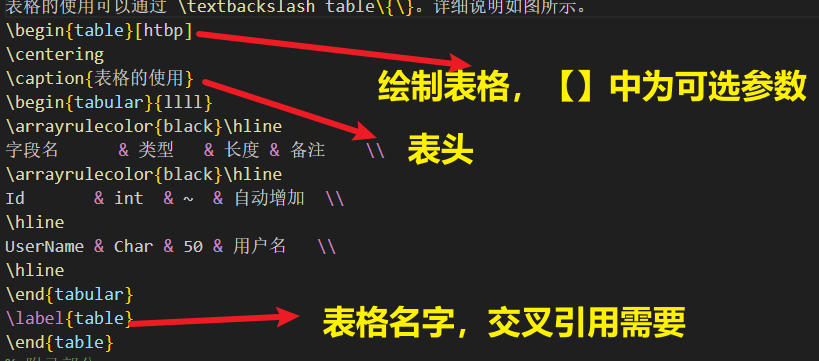
\includegraphics[width=0.65\linewidth]{image/table.png}
        \caption{表格使用}
        \label{tablea}
\end{figure}

通过绘制我们可以得到表如表\ref{table}所示。
\begin{table}[htbp]
\centering
\bicaption{示例图片：数据可视化结果}{Example Figure: Data Visualization Result}
\begin{tabular}{llll} 
\arrayrulecolor{black}\hline
字段名      & 类型   & 长度 & 备注    \\ 
\arrayrulecolor{black}\hline
Id       & int  & ~  & 自动增加  \\ 
\hline
UserName & Char & 50 & 用户名   \\
\hline
\end{tabular}
\label{table}
\end{table}

\section{公式的使用}
\begin{equation}
    q+q = 2q
    \label{gongshi}
\end{equation}
公式可通过 \textbackslash begin\{ equation \}使用，引用可通过\textbackslash label，具体操作下文会提及。

\section{图片的插入和交叉引用}
\subsection{双语标注}

可通过\textbackslash bicaption 来代替我们平时用的 \textbackslash caption,其中\textbackslash bicaption\{中文题注\}\{英文题注\}。表格与图片是使用方法同理。

\subsection{图片的使用}
图片的使用可通过\textbackslash begin\{figure\}实现，其中[htbp]可控制图片位置。见图\ref{pic}。
\begin{figure}[htbp]
        \centering
        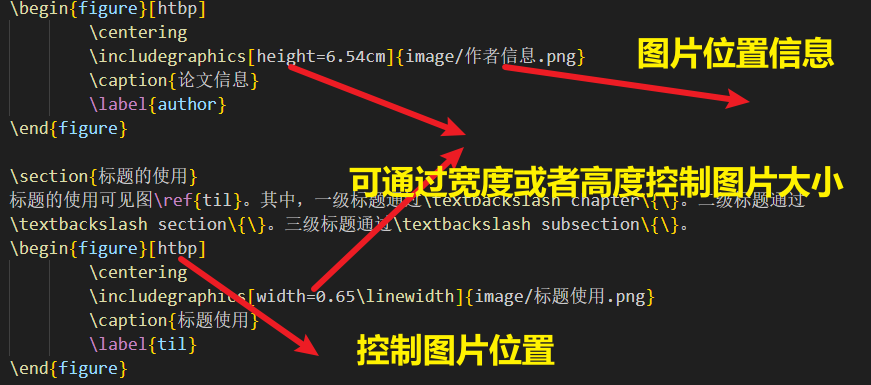
\includegraphics[width=0.65\linewidth]{image/figure.png}
        \caption{图片使用}
        \label{pic}
\end{figure}

\subsection{多图排版样例}
本章节提供几个多图摆放的样例。
\begin{figure}[htbp]
\begin{minipage}[t]{0.48\linewidth}
\centering
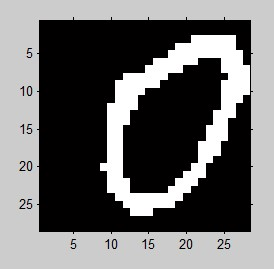
\includegraphics[width=0.9\textwidth]{image/chap04/1.jpg}
\caption{图1-1裂缝对照图}
\label{fig:side:a}
\end{minipage}%
\begin{minipage}[t]{0.48\linewidth}
\centering
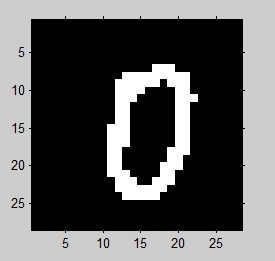
\includegraphics[width=0.9\textwidth]{image/chap04/2.jpg}  % 2.2in
\caption{图1-2裂缝对照图}
\label{fig:side:b}
\end{minipage}
\end{figure}


\begin{figure}[!htp]
	\centering
	\subfloat[附件一中图1-2]{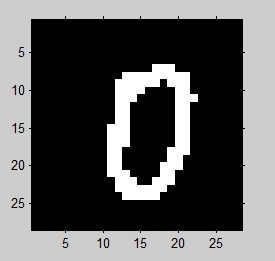
\includegraphics[width=0.4\textwidth]{image/chap04/2.jpg}}\qquad
	\subfloat[附件一中图1-8]{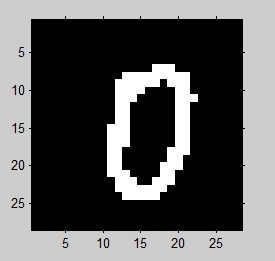
\includegraphics[width=0.4\textwidth]{image/chap04/2.jpg}} \\
	\bicaption{高斯模糊降噪后图像对比}{ddffff}
    \label{cpm-1}
\end{figure}

\subsection{交叉引用}
在\LaTeX 中，我们可以通过\textbackslash ref\{\}来对任何表格、图片、章节等进行引用。我们\textbackslash label 来对这些需要引用的命名，再在正文中通过 \textbackslash ref\{XX\}来进行引用。例如\ref{fig:side:a}，\ref{author}。但是这种方式不能自动识别图表公式，需要自行添加“图”。

已定义自动引用格式，所有引用图片、公式、表格等内容均使用同一个命令`\textbackslash autoref\{\}`进行引用，该命令将会自动产生例如` 式``图 `等前置词语。例如\autoref{cpm-1}，\autoref{author}。
\newclearpage

\chapter{参考文献说明}
参考文献的著录方法采用我国国家标准GB7714-87《文后参考文献著录规则》中规定采用的“顺序编码制”，中外文混编。论文中，引用出处按引用先后顺序用阿拉伯数字和方括号“[]”放在引文结束处最后一个字的右上角作为对参考文献表相应条目的呼应。文后参考文献表中，各条文献按在论文中的文献序号顺序排列。

参考文献引用，需按顺序引用，可利用交叉引用。其引用的文献，需采用上标字体，具体格式已在本文档做好，选中引用部分。\overcite{ref1,ref2}

参考文献均使用 bibtex 的形式记录在`main.bib`文件中，当需要引用时可使用`\textbackslash cite`和`\textbackslash overcite\`两个命令引用，前者为引用符号处于文本基线，后者为上标形式。


\newclearpage

\backmatter
\renewcommand{\chaptermark}[1]{\markboth{\songti #1}{}}
\makereferences
\newclearpage



{
    \appendix
    \renewcommand{\chaptermark}[1]{\markboth{\heiti  附录\thechapter\ ~#1}{}}
    \chapter{补充更多细节}

    \section{补充图}
    主要列入正文内过分冗长的公式推导，供查读方便所需的辅助性数学工具或表格；重复性数据图表；论文使用的缩写、程序全文及说明等。附录一般与论文全文装订在一起，与正文一起编页码，如果附录内容很多时可独立成册。若有多个附录按大写英文字母排序，如附录 A、附录B 等，每一个附录均另起一页。附录中的公式及图表编号也冠以附录序号字母加一短划线如公式A-2），图 A-2，表 B-2 等。本项可根据论文需要编排或省略。
    \subsection{补充图}

    \newclearpage
}
\ifdefined\blind  %这个if不要删除
    % 盲审版没有致谢
\else
    \chapter{致谢}

    四年时间转眼即逝，青涩而美好的本科生活快告一段落了。回首这段时间，我不仅学习到了很多知识和技能，而且提高了分析和解决问题的能力与养成了一定的科学素养。虽然走过了一些弯路，但更加坚定我后来选择学术研究的道路，实在是获益良多。这一切与老师的教诲和同学们的帮助是分不开的，在此对他们表达诚挚的谢意。

    最后我要感谢我的家人，正是他们的无私的奉献和支持，我才有了不断拼搏的信心和勇气，才能取得现在的成果。

    \vskip 108pt
    \begin{flushright}
        王小明\makebox[1cm]{} \\
        \today
    \end{flushright}
    \newclearpage
\fi
\chapter{攻读学位期间发表的研究成果}

论文格式依照《温州大学研究生学位论文格式》（温州大学行政〔2016〕153号）文件要求，上传的盲审论文含封面（盲审格式）、中英文摘要和关键词、目录、正文、参考文献、注释、附录、攻读学位期间取得的研究成果（作者、发表卷期等信息一律用“XXX”替代，详见示例）,除去扉页、版权页、致谢等部分，论文封面及论文中不得出现温州大学、指导教师及作者等相关信息,一律用“***”替代。

\ifdefined\blind  % 这个if不要删除
    % 盲审版不透露自己姓名
    \begin{enumerate}
        \renewcommand{\labelenumi}{[\arabic{enumi}]}
        \setlength{\itemindent}{0em}
        \setlength{\labelsep}{0.5em}
  
        \item XXX[J]. Journal of Materials Science-Materials in Electronics,2022,X(X): XXXX -XXXX.SCI收录，已发表，第三章的研究成果.
        \item  XXX, XXX, XXX[J]. Journal of Physics: Conference Series.2021.X(X)(本人第一作者).EI收录，已发表，第四章的研究成果.
    \end{enumerate}
\else
    攻读学位期间发表的学术论文目录格式同参考文献,并在最后注明刊物级别和第一完成单位名称。
    \begin{enumerate}
        \renewcommand{\labelenumi}{[\arabic{enumi}]}
        \setlength{\itemindent}{0em}
        \setlength{\labelsep}{0.5em}
  
        \item Zhang X, Yu Z, Zhao L, et al. COMPrompter: reconceptualized segment anything model with multiprompt network for camouflaged object detection[J]. Science China Information Sciences, 2025, 68(1): 112104. JCR 一区， 温州大学.
        \item Yu Z, Zhang X, Zhao L, et al. Exploring Deeper! Segment Anything Model with Depth Perception for Camouflaged Object Detection[C]//Proceedings of the 32nd ACM International Conference on Multimedia. 2024: 4322-4330. CCF-A ,温州大学.
    \end{enumerate}
\fi

\newclearpage
\end{document}